\documentclass[a4paper,12pt]{article}

\usepackage{url}
\usepackage{epsfig}
\usepackage{graphics}
\usepackage{fancyhdr}
\usepackage{subfig}
\usepackage{gensymb}
\usepackage{amsmath}
\usepackage{changepage}
\usepackage{bbold}
\usepackage{fancyhdr}

\usepackage{geometry}
 \geometry{
 a4paper,
 left=25mm,
 right=25mm,
 top=25mm,
 bottom=25mm,
 }

\graphicspath{{pictures/}}

\newcommand{\mx}{\mathbf{x}} 
\newcommand{\mX}{\mathbf{X}} 
\newcommand{\mG}{\mathbf{G}}
\newcommand{\mS}{\mathbf{S}}
\newcommand{\mH}{\mathbf{H}} 
\newcommand{\mI}{\mathbf{I}} 
\newcommand{\mK}{\mathbf{K}} 

\newcommand{\X}{\textbf{X}}
\newcommand{\G}{\textbf{G}}
\newcommand{\K}{\textbf{K}}

\newcommand{\mhalf}{\frac{1}{2}}

\title{Learning a Kernel Matrix for Nonlinear Dimensionality Reduction \\ or \\ The Semidefinite Teapot}
\author{\hspace*{-0.5cm}\begin{tabular}{ccc}
O. Elshenawy & E. W\"arnberg & M. Poletti \\ 
901009-T214 & 920118-3259 & 910312-T233 \\ 
omares@kth.se & emilwa@kth.se & poletti@kth.se 
\end{tabular}\\
\\
\begin{tabular}{cc}
A. Pettersson &J. B\"utepage \\
910129-3976  & 900924-T085\\ 
anderpet@kth.se & butepage@kth.se
\end{tabular}} 
% Normally there will not be any pictures but we want
% these so that we can connect faces to names in the course
% We also want birthdates so that we can tell people with the same
% name apart
\date{}

\pagestyle{fancy}
\setlength{\headheight}{25pt}
\fancyhf{}
\lhead{DD2434 - Machine Learning Advanced}  
\rhead{The semidefinite Teapot}  
\fancyfoot[C]{\thepage} 



% 1- Summary of the paper
% 2- How we did the SDP (our crazy Matrices representation)
% 3- SwissRoll experiment and Teapot as well, with their results, discuss our intuition of what happened
% 4- Discuss our intuition of the paper, and the method, its pros and cons


\begin{document}

\maketitle
\thispagestyle{fancy}
\begin{abstract}

\noindent In this report we present the replication and analysis of Weinberger et al. \cite{weinberger04}. In \cite{weinberger04} the authors describe a novel method for dimensionality reduction using Kernel Principal Component Analysis (KPCA). Instead of using a predetermined Kernel function, such as e.g. a Gaussian Kernel, the authors  propose to learn a Kernel matrix from the data. The construction of this matrix is based on neighbourhood relations and computed using semidefinite programming.

The method is tested on three different problems, unfolding a dataset in the form of a Swiss Roll, finding the low dimensional representation of images of a teapot from different angles and a classification problem based on handwritten digits. The results are similar to the results presented in \cite{weinberger04}, except for perhaps a slightly better performance for the classification problem. 


\end{abstract}



\clearpage

%%%%%%%%%%%%%%%%%%%%%%%%%%%%%%%%%%%%%%%%%%%%%%%%%%%%%%%%%%%%%
%%%%%%%%%%%%%%%%%%%%%%%%%%%%%%%%%%%%%%%%%%%%%%%%%%%%%%%%%%%%%
\section{Introduction}
\label{sec:intro}

In an age of Big Data and high dimensional data sets the topic of dimensionality reduction is essential for efficient data representation and machine learning. The basic idea behind dimensionality reduction methods is that the inherent structure of high dimensional data can be captured by a low dimensional representation without the loss of substantial information. 

Although the original data points can in principle be any type of data, the most common usage can be described mathematically as follows. Given a number of data points  \X \ = \{$\mx_1, \mx_2, ... \mx_m$\} $\in \mathcal{R}^n$, find a \textit{d} dimensional representation, with \textit{d} $<$ \textit{n}, which sufficiently captures the information content of the data.


% linear and KPCS
Next to linear approaches such as Principal Component Analysis (PCA) and Multidimensional Scaling (MDS), several methods for learning non-linear submanifolds have been developed. One Kernel based method, Kernel Principal Component Analysis (KPCA), maps the data into a, possibly infinite-dimensional, feature space before applying PCA. However, instead of computing the eigenvectors explicitly in this space the so called \emph{Kernel trick} is used. This allows the more feasible computation of the eigenvectors of the Kernel matrix. Here, the main problem is the choice of an appropriate Kernel function as the performance of submanifold learning depends heavily on this modelling decision.


% graph based
In graph-based methods, the data is represented as a graph, in which data points correspond to the vertices and distance relationships between these points constitute the edges, \cite{Murphy}. As distances on a manifold can reliably be computed for local neighbourhoods using normal euclidean distance, a common choice is to connect each vertex to its $k$ nearest neighbours. Given these distant relationships one can construct a similarity matrix. The desired submanifold is given by some kind of spectral decomposition of this matrix.


% SDE
The approach presented in this report, Semidefinite embedding (SDE), combines Kernel-based and graph-based methods by learning a positive semi-definite matrix constrained by the relations contained in the graph. According to Mercers theorem \cite{mercer}, this matrix can be viewed as the Kernel matrix needed for KPCA. Thus, instead of using a fixed Kernel function, the learning of the Kernel matrix preserves the local structure of the original manifold while unravelling its global complex properties.


% what we will present
In the following, we will shortly present the basic concepts of different methods for dimensionality reduction based on \cite{saul06}. Especially, we will focus on SDE and how it can be related to MDS and KPCA. After describing our implementation of SDE, we will present a number of experiments along with our results. At last, we will discuss the implications, merits and limitations of the method. 

%%%%%%%%%%%%%%%%%%%%%%%%%%%%%%%%%%%%%%%%%%%%%%%%%%%%%%%%%%%%%
%%%%%%%%%%%%%%%%%%%%%%%%%%%%%%%%%%%%%%%%%%%%%%%%%%%%%%%%%%%%%
\section{Methods for dimensionality reduction}
\label{sec:relwork}

%---------------------------------------------------------------------------------------------------------------------------------------------------------------------
\subsection{Linear Methods}
\label{sec:LinMet}
% summary PCA
One of the basic approaches is Principal Component Analysis (PCA). In order to maximize the information retained by the subspace, it is constructed of \textit{d} basis vectors that capture the directions of maximal variance in the original data. The solution to this problem are \textit{d} eigenvectors corresponding to the \textit{d} largest eigenvalues of the covariance matrix of \X, \cite{Murphy2}.

%summary MDS
Another linear approach is Multidimensional Scaling (MDS) which attempts to find a representation that preserves distance relationships between data points in the original space. As the aim is to minimize the squared difference of  dot products of \X \  in both the original and the low dimensional representation, the solution is given by the spectral decomposition of the Gram matrix \G, with \G$_{ij} = \mx_i^T \mx_j$. This matrix can be derived by a transformation of the distance matrix \textbf{S}, with 
S$_{ij} = || \mx_i - \mx_j || ^2$, as \G = $-\mhalf \mH\mS\mH$, where $ \mH  = \mI - \frac{1}{n}(1,1, ..., 1)^T(1,1, ..., 1)$. This construction is feasible if the inputs are centered. In the following, the \textit{d} dimensional subspace, \textit{d} $\leq$ \textit{n},  is constructed of \{$\sqrt{\lambda_i}\mathbf{e}_i\}_{i = \{1,..d\}}$, where $\mathbf{e}_i$ is the ith eigenvector of \G \ corresponding to the ith eigenvalue $\lambda_i$ and \textit{d} is the number of large eigenvalues, \cite{Williams}.

%---------------------------------------------------------------------------------------------------------------------------------------------------------------------
\subsection{Kernel PCA}

The linear methods above can be extended to non-linear problems by mapping the input vectors \X \ into a feature space $(\Phi(\mx_1), \Phi(\mx_2), ... \Phi(\mx_n)) \in \mathcal{H}$, where $\mathcal{H}$ lives in  possibly infinite dimensions. Instead of constructing a covariance matrix in $\mathcal{H}$, the "Kernel trick" can be applied. For centred data the covariance matrix \K \ is given by the point-wise dot product of the data points in the feature space with \K$ = \frac{1}{n}\sum_{i = 1}^n \Phi(\mx_i)   \Phi(\mx_i)^T$.  The zero mean assumption made above implies, that we must subtract the mean in the feature space. Therefore, the construction of \K \ resembles the centred construction of the Gram matrix explained for MDS in Sec. \ref{sec:LinMet}. The final Kernel matrix is given by \K \ = $-\mhalf \mH\mathbf{K}\mH$, where $ \mH  = \mI - \frac{1}{n}(1,1, ..., 1)^T(1,1, ..., 1)$. Finally, the eigendecomposition of \K \ yields the lower dimensional space based on the non-linear feature space. 
As a result, Kernel PCA resembles MDS where the distances between data points are represented in a feature space instead of assumed Euclidean distances, \cite{Murphy3}.

For predefined Kernel mappings, such as the squared exponential Kernel $K(\mx_i,\mx_j) = e^{\frac{-|\mx_i - \mx_j|^2}{2*\sigma^2}}$ or polynomial $K(\mx_i,\mx_j) = ( 1 + \mx_i^T\mx_j)^p$, this method produces no satisfying results for manifold learning. Instead, the choice of the Kernel influences the final mapping from higher to lower dimensions drastically. This implies that the manifold is not unfolded but that the data is mapped onto the space that is enforced by the Kernel function, as can be seen in \cite{weinberger04}.

%---------------------------------------------------------------------------------------------------------------------------------------------------------------------
\subsection{Semidefinite embedding}
\label{SDem}
In order to ensure an unfolding of the high dimensional manifold, Weinberger et al. \cite{weinberger04} introduced a method to learn a positive semidefinite Kernel matrix \K \ that guarantees maximal variance for the principle directions  in the feature space. The goal is to learn a centered, positive semidefinite matrix $\mK$ which preserves local neighbourhood relations while enforcing high global variance. This optimization problem is defined over the cone of positive semidefinite matrices with a single optimum, thus resembling a convex optimization problem. In the following, these constraints will be discussed in more detail.

A positive semidefinite matrix is given, when all eigenvalues are larger or equal to zero. In order to provide a valid solution for dimensionality reduction methods and as a requirement for Kernel matrices in general, $\mK$ has to be positive semidefinite.

Secondly, the inner products of the features need to be centered if $\mK$ is supposed to represent a covariance matrix that can be used for dimensionality reduction. So, we require
\begin{equation}
0 = |\sum_{i = 1}^n\Phi(\mx_i)|^2 = \sum_{i = 1}^n\sum_{j = 1}^n\Phi(\mx_i)\Phi(\mx_j) =  \sum_{i = 1}^n\sum_{j = 1}^n \mK_{ij},
\end{equation}
which is a linear constraint that preserves the convexity of the optimization.

The final goal is to unfold the underlying manifold and reveal a lower dimensional submanifold. Therefore, local neighbourhood relations need to be preserved. The transformation between the manifolds can be regarded as a locally isotropic mapping if $\Phi(\mx_i)$ can be derived by a translation and rotation of $\mx_i$.

Let the binary matrix $\mathbf{\eta}$ define the neighbourhood relationships between each pair $\{(\Phi(\mx_i),\Phi(\mx_j))\}_{ij}$, where $\mathbf{\eta}_{ij} = 1$ if $\Phi(\mx_i)$ and $\Phi(\mx_j)$ are neighbours and $\mathbf{\eta}_{ij} = 0$ otherwise. In order to determine these relationships the $k$ nearest neighbours of each point can be determined using Euclidean distances. Note that this definition means that $\mathbf{\eta}_{ij} = 1$ does not necessarily imply that $\mathbf{\eta}_{ji} = 1$. For each $\eta_{ij} = 1$, the local distance in the original space and the feature space should be equal, which can be stated as 

\begin{equation}
|\Phi(\mx_i) - \Phi(\mx_j)|^2 = |\mx_i - \mx_j|^2 \label{Eq:dist}
\end{equation}
Given that $\mG$ is the Gram matrix in the original space with \G$_{ij} = \mx_i^T \mx_j$ and $\mK$ is constructed of inner products in the feature space %transformed space?
with \K$_{ij} = \Phi(\mx_i)^T \Phi(\mx_j)$, the requirement in Eq. \ref{Eq:dist} can be expressed in terms of single inner products
\begin{equation}
\mK_{ii} + \mK_{jj} - \mK_{ij} - \mK_{ji}  = G_{ii} + G_{jj} - G_{ij} - G_{ji}. 
\end{equation}
This is again a linear constraint supporting convex optimization.

Given this set of constraints, the optimization aims to increase the variance in the principle directions of the feature space. Thus, the pairwise distance between feature vectors has to be maximized. This results in the maximization of 
\begin{align}
\frac{1}{2N}\sum_{i = 1}^n\sum_{j = 1}^n |\Phi(\mx_i) - \Phi(\mx_j)|^2 =  \frac{1}{2N}\sum_{i = 1}^n\sum_{j = 1}^n \mK_{ii} + \mK_{jj} - 2 \mK_{ij} = Tr(\mK)
\end{align}

In conclusion, the learning of a Kernel matrix can be formalized as the following positive semidefinite optimization problem:\\
Maximize the trace Tr(\K) under the constraints
\begin{align}
\label{eq1}1.& \ \mK\succeq 0 \text{, semidefinite positive}\\
\label{eq2}2.& \ \sum_{i = 1}^n\sum_{j = 1}^n \mK_{ij} = 0\\
\label{eq3}3.&  \ \mK_{ii} + \mK_{jj} - \mK_{ij} - \mK_{ji}  = \mG_{ii} + \mG_{jj} - \mG_{ij} - \mG_{ji}\\
& \text{for all i,j such that } \eta_{ij} = 1 \ \text{or}\ [\eta^T\eta]_{ij} > 0 \nonumber 
\end{align} 

To the resulting matrix, Kernel PCA can be applied in order to extract the principal components describing the mapping of the data onto a lower dimensional submanifold. 

\subsection{Intuitive interpretation}
The above constraints can be interpreted physically in a rather intuitive fashion. In order to have as large variance between the data points as possible, we want the submanifold to be maximally unfolded. The goal function of the optimization can thus be seen as having forces trying push apart the data points. However, the neighbour-constraints (Eq. \ref{eq3}) prevents these forces from tearing apart the submanifold. Equation \ref{eq1} ensures that these forces causes physically reasonable movements by requiring that the gram matrix, created from their position vectors, is valid. Equation \ref{eq2} is simply a convenience required for the kernel trick to work, but can be seen as keeping the mass center of the manifold at the origin throughout the unfolding process.

In the light of this intuition it is easy to explain the behaviour of the algorithm under certain conditions. For example, if the data is so that the manifold consists of two (or more) pieces they can be forced arbitrarily far away for each other --- the optimization becomes unbounded. Similarly, if two points from different parts of the manifold accidentally becomes neighbours this sews together the two parts making it impossible to unfold them completely.
%%%%%%%%%%%%%%%%%%%%%%%%%%%%%%%%%%%%%%%%%%%%%%%%%%%%%%%%%%%%%
%%%%%%%%%%%%%%%%%%%%%%%%%%%%%%%%%%%%%%%%%%%%%%%%%%%%%%%%%%%%%
\section{Our approach}
\label{sec:method}
As in the original work we have used the SeDuMi MATLAB optimization toolbox. It requires formulating the problem into a Standard Dual Problem (SDP). The general form of SDP as represented in SeDuMi is, see \cite{SeDuMi}:
\begin{align}
\textnormal{minimize :}~& c^T y \\
\textnormal{subject to :}~& \mathbf{A}y \ge b \\
~& F_0 + y_1 F_1 + ... + y_n F_n\succeq 0
\end{align}
where $F_0 = diag(b)$, $F_i = diag(a_i) \textnormal{ for } \forall i = 1...n$ and $\mathbf{A} = [a_1 . . . a_n] \in \mathcal{R}^{m * n}$. 
We represented the constraints on \K, see Eq. \ref{eq1},\ref{eq2}, and \ref{eq3}, as follows.

$y$ in the SeDuMi constraints corresponds to our Kernel matrix $\mK$. Since we were interested in optimizing only the trace, we chose $c$ to be the Identity matrix, reshaped to a column vector because SeDuMi expects all inputs to be in vector form.

In order to determine neighbouring points, $\eta$ was determined by choosing the k nearest neighbours as described in Sec. \ref{SDem}. The matrix $\mathbf{A}$ was carefully designed to select elements from $\mK$ that corresponded to the third constraint, i.e. to enforce $\mK_{ii} + \mK_{ij} - \mK_{ij} - \mK_{ji}$ where $\eta+\eta^T\eta$ is non-zero, Thus, $\mathbf{A}$ was of size $N$ by $M^2$, where $N = \sum_{ij}^M{\mathbb{1}([\eta+\eta^T\eta]_{ij} > 0)}$ and $M$ is the number of data points. Here, $\mathbf{A}$ was a sparse matrix whose rows represent the left side of Eq. \ref{eq3} whenever applicable. The entry 1 was assigned to the indices $ii$ and $ij$ and the entry -1 to $ij$ and $ji$ respectively. Since the Gram matrix $\mG$ is constant, we pre-calculated the values constituting the right side of Eq. \ref{eq3} and assigned these to $b$. To satisfy Eq. \ref{eq2}, $\mathbf{A}$ was augmented with an extra row containing only 1s and $b$ with an extra zero entry. The final dimensionality of $\mathbf{A}$ was N+1 times $M^2$, and $b$ was a vector of size N+1.

For the first constraint, the SeDuMi toolbox has a parameter that is set in its option struct to ensure positive semidefiniteness during the optimization.


%%%%%%%%%%%%%%%%%%%%%%%%%%%%%%%%%%%%%%%%%%%%%%%%%%%%%%%%%%%%%
%%%%%%%%%%%%%%%%%%%%%%%%%%%%%%%%%%%%%%%%%%%%%%%%%%%%%%%%%%%%%
\section{Experiments}
\label{sec:exps}



%---------------------------------------------------------------------------------------------------------------------------------------------------------------------
\subsection{Setup}
We performed the experiments on different data sets to confirm the findings of Weinberger et al. \cite{weinberger04}. Two types of experiments were conducted: First, we tested the performance of the SDE Kernel in manifold  learning, then we investigated the efficacy of SDE in large margin classification. In both cases, we compared the performance of SDE to linear, polynomial and Gaussian Kernels.

To test manifold learning we used two data sets. The first dataset was a three dimensional “Swiss Roll” with 500 data points. The second dataset consisted of 100 images representing a rotating teapot. Here, each data point was an image of the teapot viewed from a different angle equally spaced in $[0^{\circ},360^{\circ}]$. Each image was represented by 76 x 101 pixels where each pixel was encoded in three colour bytes. All the experiments were run with $k = 4$, the number of neighbours. The efficacy was evaluated considering the dimensionality of the transformed data points expressed by the the number of significant eigenvalues found: the closer the number of dimensions found was to the intrinsic number of dimensions of the manifold, the better the method performed.

To evaluate the large margin classification behaviour of the SDE Kernel, we used a set of handwritten digits. A binary classification problem consisting of two distinct digits had to be solved by a support vector classifier using all four Kernels respectively. To test the performance, we applied a 10-fold cross validation on a training set (N = 810) and a test dataset (N = 90). The SDE Kernel matrix was learned on the whole dataset while ignoring the labels, while the testing was solely based on the testing data.  


%--------------------------------------------------------------------------------------------------------------------------------------------------------------------- 

\begin{figure}[t!]
\centering
\begin{tabular}{ccc}
\subfloat[ ]{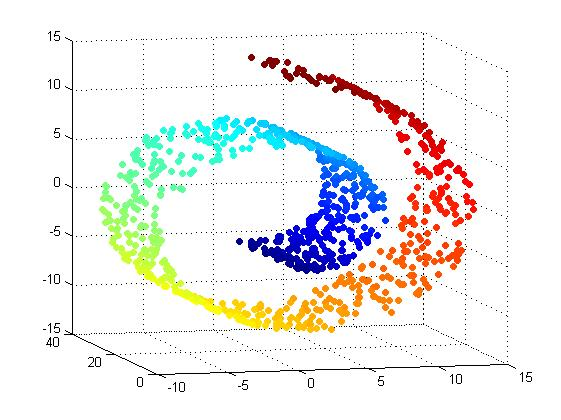
\includegraphics[scale = 0.2   ]{niceSwissRoll.jpg}} &
\subfloat[ ]{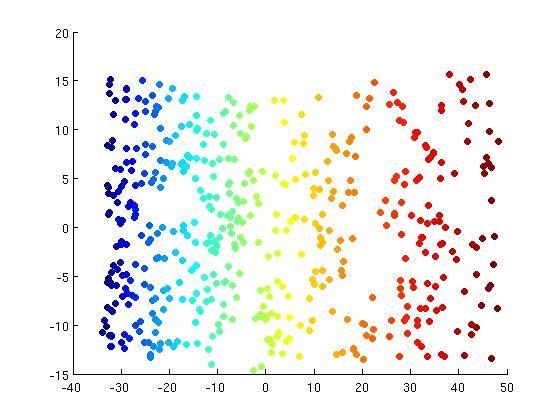
\includegraphics[scale = 0.2  ]{SwissRoll.jpg}}&
\subfloat[]{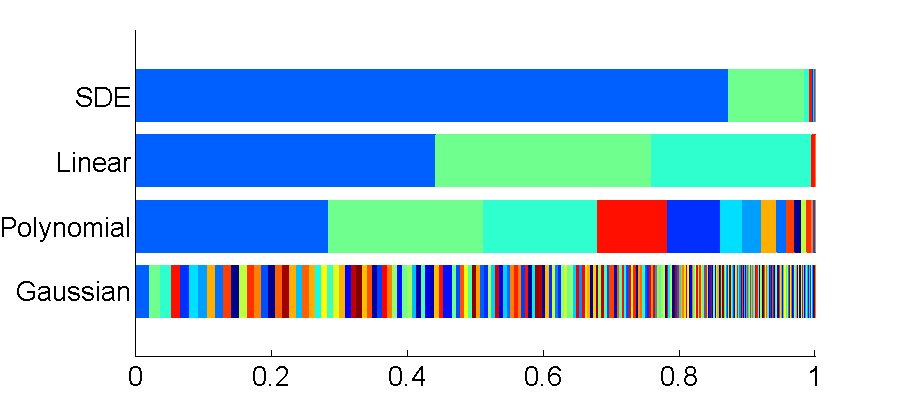
\includegraphics[scale = 0.2  ]{StackedBarSwissRoll.png}}
\end{tabular}
\caption{\small{Figures displaying the results for the Swiss Roll problem. a)Swiss Roll in the original dimension. b) Swiss Roll in the lower dimension. c) Normalized eigenvalues of the different kernel matrices (from top: SDE, linear, polynomial, Gaussian). polynomial: $p=4$ and $Gaussian: \sigma = 1.9979$}}
\label{fig:Swiss}
\end{figure}

\subsection{Results}

The results for the first task, the Swiss Roll, can be found in Fig. \ref{fig:Swiss}. In Fig. \ref{fig:Swiss}a) we see that the data can be described by two only dimensions. This unfolding is achieved by the SDE Kernel and visualized in Fig. \ref{fig:Swiss}b). Fig. \ref{fig:Swiss}c) displays the normalized eigenvalues of the respective Kernel matrices. It shows that the SDE Kernel has two large eigenvalues, which reliably approximate the true nature of the data. This feature is not captured by any of the other Kernels, since they demonstrate several relatively equally large eigenvalues. This corresponds well to the results in \cite{weinberger04}.

For the teapot problem, the result is found in Fig. \ref{fig:Tea}. Since the teapot was photographed from several possible angles, the set of images has actually only a single degree of freedom, the angle of rotation. This is captured by the principal directions of the SDE Kernel matrix, see  Fig. \ref{fig:Tea}a) and c). For a $360^{\circ}$ rotation, the algorithm places the data points on a circle and a $180^\circ$ rotation results in a line. In Fig. \ref{fig:Tea}b) and d) we see that we have one and two significant eigenvalues respectively. As before, the other kernels are not able to discover this low dimensional representation. Once again the result corresponds well to the results in \cite{weinberger04}.

\begin{figure}[t!]
\centering
\begin{tabular}{cccc}
\subfloat[]{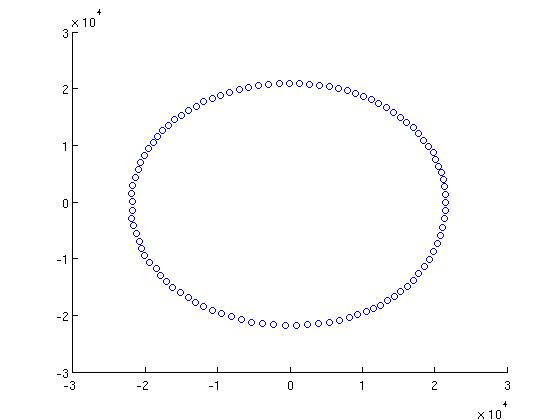
\includegraphics[scale = 0.2   ]{teapotLowAll.jpg}} &
\subfloat[]{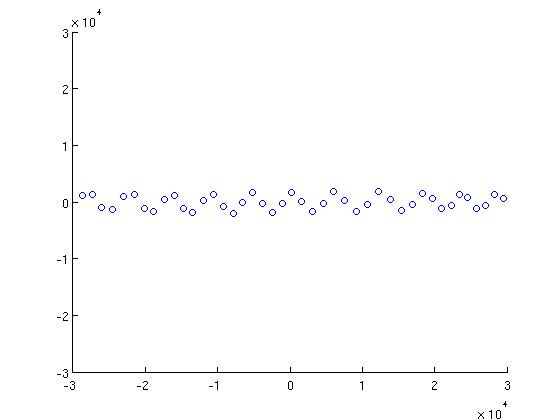
\includegraphics[scale = 0.2  ]{teapotLowHalf.jpg}}\\
\subfloat[]{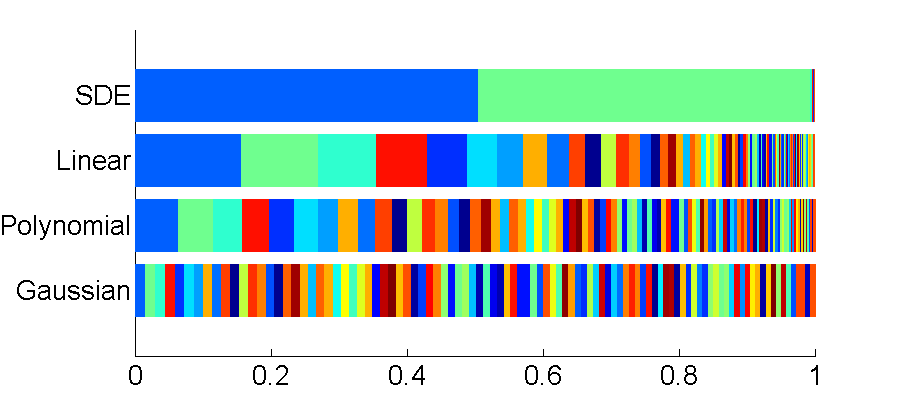
\includegraphics[scale = 0.26   ]{StackedBarTea360.png}} &
\subfloat[]{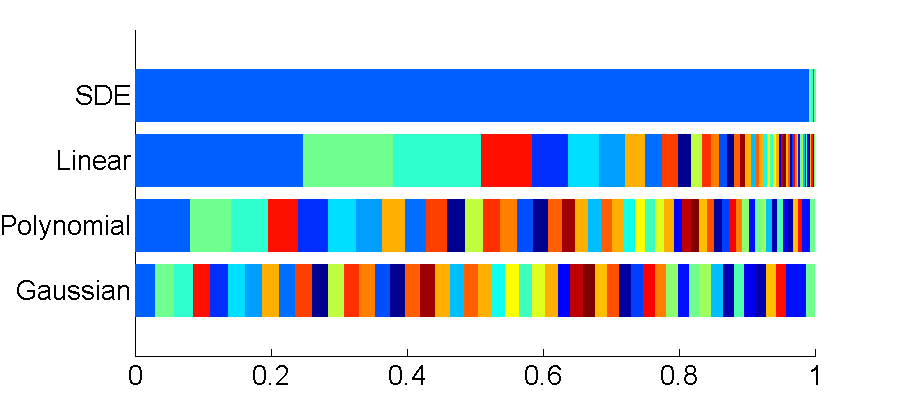
\includegraphics[scale = 0.266   ]{StackedBarTea180.png}}
\end{tabular}
\caption{\small{Figures displaying the results for the Teapot problem. a) All teapots (0-360$^{\circ}$) after unfolding. b) Half of the teapots (0-180$^{\circ}$ after unfolding. c) Normalized eigenvalues corr. to a) (from top: SDE, linear, polynomial, Gaussian), polynomial: $p=4$ and Gaussian: $\sigma = 1541$ d) Normalized eigenvalues corr. to b) (from top: SDE, linear, polynomial, Gaussian), polynomial: $p=4$ and Gaussian: $\sigma = 1541$}}
\label{fig:Tea}
\end{figure}


For the classification problem, we first studied the eigenvalues for each Kernel matrix when applying it to a classification task between the digits 2 and 3, see Fig.\ref{fig:Class}a). SDE assigns more importance to a small number of eigenvalues, than the other Kernels where information is distributed over several dimensions. This result is similar to the result achieved in \cite{weinberger04}. Table \ref{fig:Class}b) displays the error rates for different pairs of digits, determined with cross-validation. These error rates suggest that the SDE performs worse compared to the other Kernels for some digits. Nevertheless, the result for our SDE Kernel seem significantly better than the result for the SDE in \cite{weinberger04}, while our polynomial Kernel performs slightly worse. The performance of both the polynomial and the Gaussian Kernel depend heavily on the choice of parameters. Given a different data set, the parameters are likely to change which might explain the discrepancy.   



\begin{figure}
\centering
\begin{tabular}{cc}
\subfloat[]{\raisebox{-.40\height}{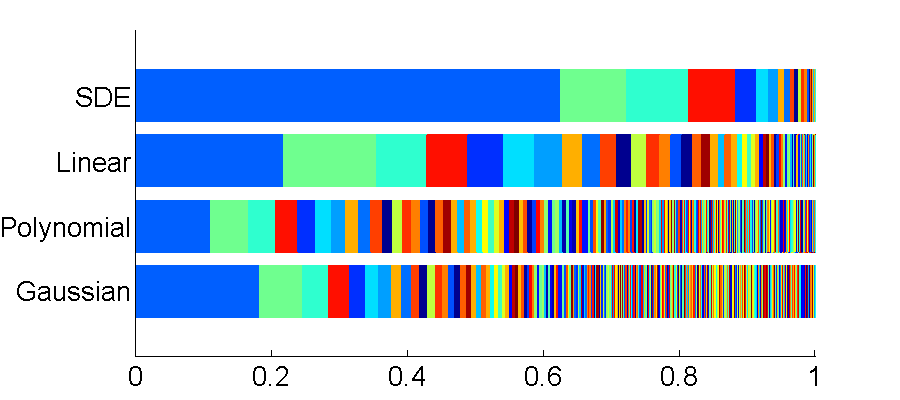
\includegraphics[scale=.26]{StackedBarLargeMargin2vs3}}}
\label{fig:Class} & 
\subfloat[]{
\begin{footnotesize}
   \begin{tabular}{ | c | c | c | c | c |}
    \hline  
    Digits & Linear & Polynomial & Gaussian & SDE\\ \hline
    1 vs 2 & 0.4444 & 0.5556 & 0.4444 & 0.8889 \\ \hline
    1 vs 3 & 0 & 0.1111 & 0.1111 & 0.1111 \\ \hline
    2 vs 8 & 2.6667 & 2.000 & 1.1111 & 1.2222 \\ \hline
    8 vs 9 & 0.7778 & 3.1111 & 0.3333 & 1.4444 \\ 
    \hline
  \end{tabular} 
   \end{footnotesize}}
\end{tabular}
\caption{Results of the large margin classification. a) Normalized eigenvalues for the digits 2 and 3 (from top: SDE, linear, polynomial, Gaussian) with N = 802, polynomial: $p=2$ and Gaussian: $\sigma = 5.3651$ b) Classification error, in percent, of the different Kernels for pairs of digits. Polynomial $p=2$ and Gaussian: $\sigma$ = average distance between neighbouring points. }\label{fig:Class}
\end{figure}

%------------------------------------------------------------------------------------------------------------------

\subsection{Additional Observations}
\begin{figure}
\centering
\subfloat[]{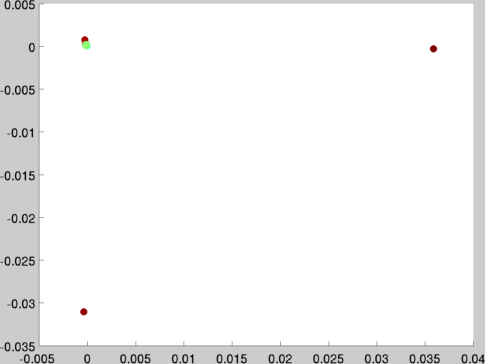
\includegraphics[scale=0.3]{pictures/CarlK1.png}}~
\subfloat[]{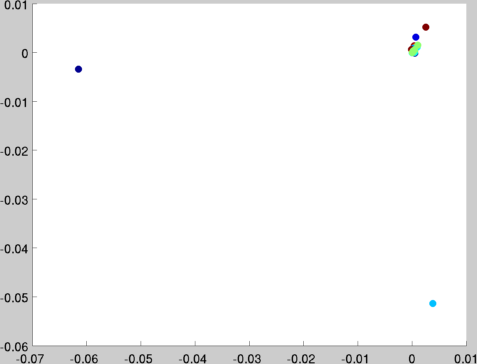
\includegraphics[scale=0.3]{pictures/CarlK2.png}}~
\subfloat[]{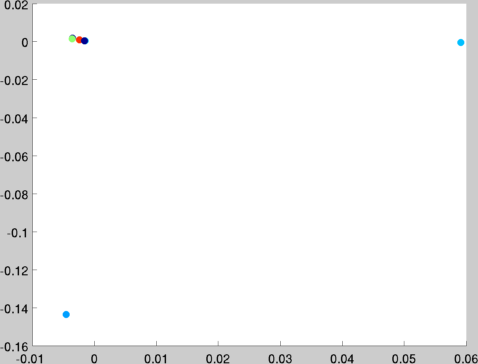
\includegraphics[scale=0.3]{pictures/CarlK3.png}}~
\subfloat[]{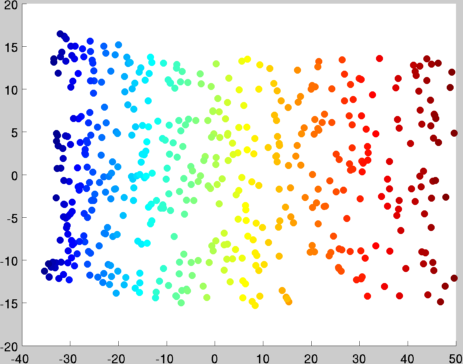
\includegraphics[scale=0.3]{pictures/CarlK4.png}}\\

\subfloat[]{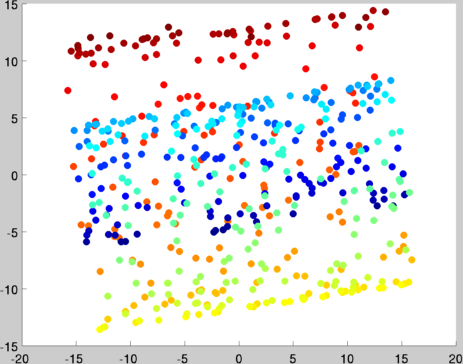
\includegraphics[scale=0.3]{pictures/CarlK5.png}}~
\subfloat[]{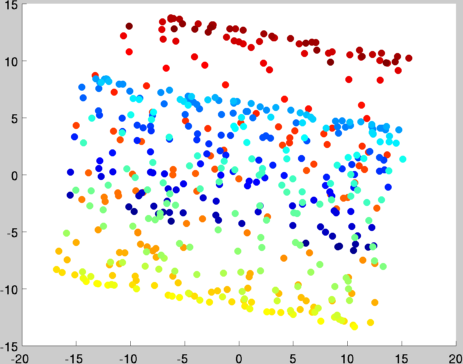
\includegraphics[scale=0.3]{pictures/CarlK6.png}}~
\subfloat[]{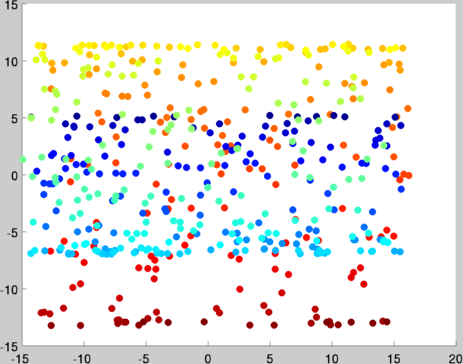
\includegraphics[scale=0.3]{pictures/CarlK8.png}}
\caption{Projections using different K values, from top left to bottom right: K=1,2,3,4,5,6 and 8.}
\label{fig:DifferentKs}
\end{figure}

We have also investigated how changing some hyper parameters affect the problem.
\subsubsection{Swiss Roll}
We have run with different K sizes for a fixed size N=500, as we can see in Figure~\ref{fig:DifferentKs}, with a very small K (K=1,2 and 3), the neighbourhood relationship is limited, therefore $\eta + \eta^T\eta$ is very sparse, and that means a small number of points will be considered for the optimization, which is kind of similar to the problem of the data being disjoint. However this is influenced by N, for N=100, K=3 was able to unroll correctly.
With a larger K, the optimization fails to unfold, resulting in the shape in \ref{fig:DifferentKs} and 3 large eigenvalues, it is as if the roll was just projected into two dimensional space. The intuition behind this is that the points are connected to false neighbours, this can be imagined as very strong glue at the curves of the Swiss Roll, therefore, trying to unfold it, would be like unfolding a spring, there will be a lot of resistance.

\subsubsection{Teapot}
\begin{figure}
\centering
\subfloat[]{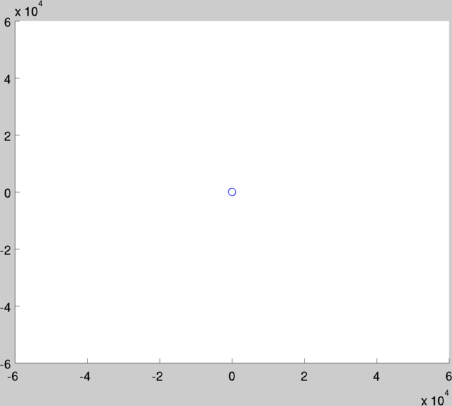
\includegraphics[scale=0.3]{pictures/TeapotK1.png}}~
\subfloat[]{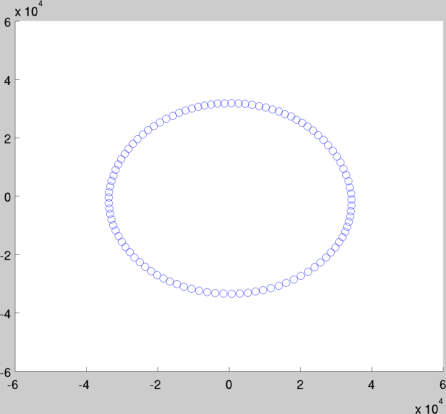
\includegraphics[scale=0.3]{pictures/TeapotK2.png}}~
\subfloat[]{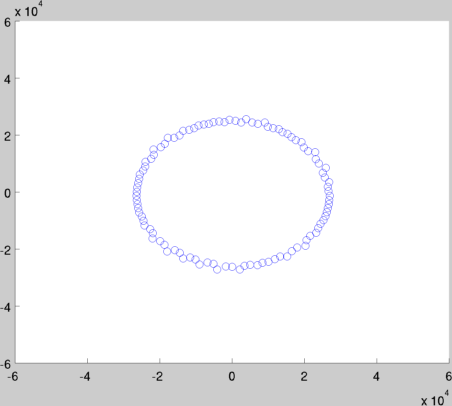
\includegraphics[scale=0.3]{pictures/TeapotK3.png}}~
\subfloat[]{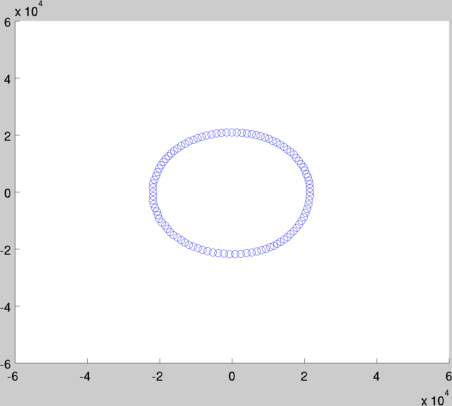
\includegraphics[scale=0.3]{pictures/TeapotK4.png}}\\

\subfloat[]{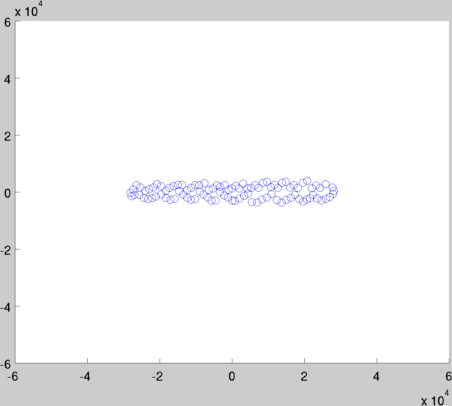
\includegraphics[scale=0.3]{pictures/TeapotK5.png}}~
\subfloat[]{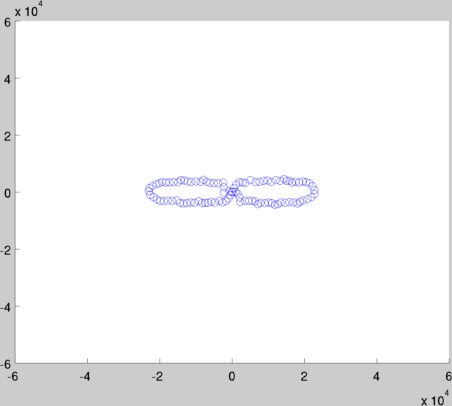
\includegraphics[scale=0.3]{pictures/TeapotK6.png}}~
\subfloat[]{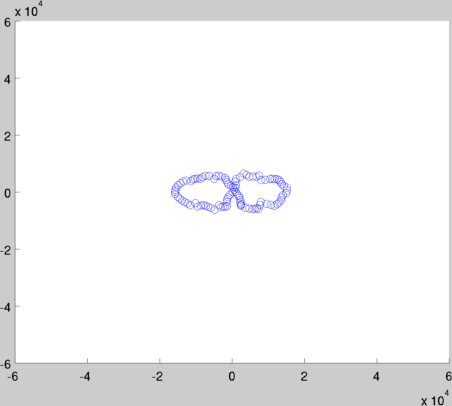
\includegraphics[scale=0.3]{pictures/TeapotK8.png}}
\caption{Projections using different K values, from top left to bottom right: K=1,2,3,4,5,6 and 8.}
\label{fig:TeapotKs}
\end{figure}
Changing K along with the teapot dataset has shown similar behaviour to that of the Swiss Roll. This is clearly seen in Figure~\ref{fig:TeapotKs}. When false neighbours start to get into the picture, the unfolding becomes very difficult.


%%%%%%%%%%%%%%%%%%%%%%%%%%%%%%%%%%%%%%%%%%%%%%%%%%%%%%%%%%%%%
%%%%%%%%%%%%%%%%%%%%%%%%%%%%%%%%%%%%%%%%%%%%%%%%%%%%%%%%%%%%%
\section{Discussion}
\label{sec:summary}
Given a functioning optimizer for positive semidefinite matrices, we found the implementation of SDE to be rather straight forward. Furthermore, we have successfully verified the claims of performance presented in \cite{weinberger04}. For the tasks with the Swiss Roll and the Teapot, the algorithm outperforms the other Kernel methods, as in \cite{weinberger04}. While for the classification problem the SDE performs worse than the other Kernel methods in some cases, but perhaps not as badly as in \cite{weinberger04}.  

The relative ease of implementation and the performance on benchmark problems makes SDE a powerful method. However, there are some severe limitations to its use. To begin with, we found that having too few data points reduced robustness by jeopardizing the connectedness of the neighbourhood graph. SDE requires that there is a sufficiently dense amount of data points throughout the entire sub-manifold. On the other end, the considerable computational resources required limits its practical use for large datasets. In combination, these two limitations restricts SDE's practical use to contexts ranging from a few hundred to a couple of thousands data points. Even for such a simple example as the Swiss Roll, the level of noise has a large impact on the performance of SDE as the assumption of local neighbourhoods is not satisfied.

%The experiments presented in this report are however not sufficient to specify these limits further nor to describe their dependence on the type of data.  ? really ?

One of the key strengths of SDE is that the Kernel values are optimized globally. Nevertheless, this property also introduces a few problems. For instance, if the algorithm is used in some kind of online context, this requires the entire Kernel matrix to be recomputed for each addition of data. This disables the possibility of separating a computationally heavy learning phase from a quick classification/evaluation phase. For classification, it also implies that a set of evaluation points could be classified differently depending on whether they are evaluated collectively or separately. In fact, the introduction of a single evaluation point could potentially alter the classification boundaries completely. For example, a single data point in the teapot problem, the last one to close the loop constitutes the boundary between the output of a circle or a line. The feature space changes from essentially one-dimensional to two-dimensional depending on only one data point. Whether this behaviour is desirable could be discussed and naturally depends on the context. Nevertheless, it is a fundamentally different behaviour than other Kernels used in for example Support Vector Machines.

In conclusion, the properties of the SDE can be said to make it useful for slightly different settings than ordinary KPCA. Hence, one might question the validity of comparing it straight off to polynomial or Gaussian Kernels. As stated in Sec. \ref{sec:intro}, SDE can be seen as a combination of Kernel based and graph based methods. Therefore, a fair evaluation of the merits of SDE should also include a comparison to other graph-based methods. One example of such a method is \emph{Isomap}, which is mentioned by Weinberger et al. We made a preliminary implementation which ran considerably faster than SDE on the same problem set while still performing comparably well. However, an extensive comparison between these methods is beyond the scope of this report.

SDE has displayed fantastic results for some problems, but the range of applications for the method is severely limited. This in mainly because the optimization requires the dataset not be too spread-out and to fulfill the criterion of connectedness. Additionally, if there is a lot of data the optimization will be very computationally heavy. Finally, the ideal choice of $k$ seem to be dependent on the specific problem at hand. However, these flaws could possibly be dealt with and in \cite{weinberger04} they suggest several improvements of the method, such as using faster optimization algorithms, changing the optimization criteria to add slack and replacing the objective function.    

%%%%%%%%%%%%%%%%%%%%%%%%%%%%%%%%%%%%%%%%%%%%%%%%%%%%%%%%%%%%%
%%%%%%%%%%%%%%%%%%%%%%%%%%%%%%%%%%%%%%%%%%%%%%%%%%%%%%%%%%%%%
\bibliographystyle{plain}
\bibliography{reflist}


\end{document}


\begin{figure}[h!]
\center
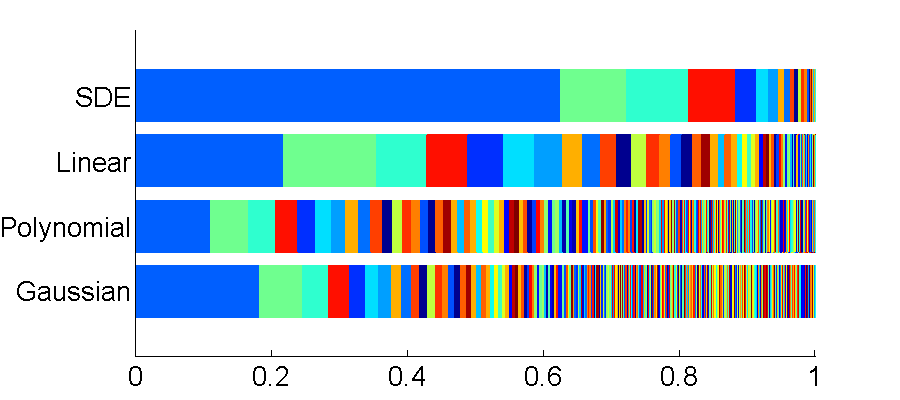
\includegraphics[scale=.45]{StackedBarLargeMargin2vs3}\\
\caption{Normalized eigenvalues of the different kernel matrices for the classification problem and the digits 2 and 3. The sample size was 802. For the polynomial kernel $p=2$ and $\sigma = 5.3651$ for the Gaussian kernel. }
\label{fig:Class}
\end{figure}


\begin{table}[h!]
\begin{center}
  \begin{tabular}{ | c | c | c | c | c |}
    \hline
    Digits & Linear & Polynomial & Gaussian & SDE\\ \hline
    1 vs 2 & 0.4444 & 0.5556 & 0.4444 & 0.8889 \\ \hline
    1 vs 3 & 0 & 0.1111 & 0.1111 & 0.1111 \\ \hline
    2 vs 8 & 2.6667 & 2.000 & 1.1111 & 1.2222 \\ \hline
    8 vs 9 & 0.7778 & 3.1111 & 0.3333 & 1.4444 \\ 
    \hline
  \end{tabular}
\end{center}
\caption{The error rates in percent for SVM classification using
different kernels on test sets of handwritten digits. Each
line represents the average of 10 experiments, where the dataset was splited of training and testing data, 90\% for training and 10\% for testing. $p=2$ for the polynomial kernel and $\sigma$ for the Gaussian kernel was taken as the mean distance between the points in that particular dataset.}
\label{tab:Class}
\end{table}
